\pdfminorversion=4 % for acroread
%\documentclass[aspectratio=169,t,xcolor={usenames,dvipsnames}]{beamer}
\documentclass[aspectratio=169,t,handout,xcolor={usenames,dvipsnames}]{beamer}
\usepackage{../beamerstyle}
\usepackage{dsfont}
\usepackage{bm}
\usepackage[english]{babel}
\usepackage[utf8]{inputenc}
\usepackage{graphicx}
\usepackage{algorithm}
\usepackage[ruled,vlined,algo2e,linesnumbered]{algorithm2e}
%\usepackage[boxed,vlined]{algorithm2e}
\usepackage{hyperref}
\usepackage{booktabs}
\usepackage{mathtools}

\usepackage{amsmath,amssymb}
\usepackage{listings}
\lstset{frame=lines,framesep=3pt,numbers=left,numberblanklines=false,basicstyle=\ttfamily\small}

\usepackage{subfig}
\usepackage{multicol}
%\usepackage{appendixnumberbeamer}
%
\usepackage{tcolorbox}

\usepackage{pgfplots}
\usepackage{tikz}
\usetikzlibrary{trees} 
\usetikzlibrary{shapes.geometric}
\usetikzlibrary{positioning,shapes,shadows,arrows,calc,mindmap}
\usetikzlibrary{positioning,fadings,through}
\usetikzlibrary{decorations.pathreplacing}
\usetikzlibrary{intersections}
\usetikzlibrary{positioning,fit,calc,shadows,backgrounds}
\pgfdeclarelayer{background}
\pgfdeclarelayer{foreground}
\pgfsetlayers{background,main,foreground}
\tikzstyle{activity}=[rectangle, draw=black, rounded corners, text centered, text width=8em]
\tikzstyle{data}=[rectangle, draw=black, text centered, text width=8em]
\tikzstyle{myarrow}=[->, thick, draw=black]

% Define the layers to draw the diagram
\pgfdeclarelayer{background}
\pgfdeclarelayer{foreground}
\pgfsetlayers{background,main,foreground}

%\usepackage{listings}
%\lstset{numbers=left,
%  showstringspaces=false,
%  frame={tb},
%  captionpos=b,
%  lineskip=0pt,
%  basicstyle=\ttfamily,
%%  extendedchars=true,
%  stepnumber=1,
%  numberstyle=\small,
%  xleftmargin=1em,
%  breaklines
%}

 
\definecolor{blue}{RGB}{0, 74, 153}

\usetheme{Boadilla}
%\useinnertheme{rectangles}
\usecolortheme{whale}
\setbeamercolor{alerted text}{fg=blue}
\useoutertheme{infolines}
\setbeamertemplate{navigation symbols}{\vspace{-5pt}} % to lower the logo
\setbeamercolor{date in head/foot}{bg=white} % blue
\setbeamercolor{date in head/foot}{fg=white}
\setbeamercolor{author  in head/foot}{bg=white} %blue
\setbeamercolor{title in head/foot}{bg=white} % blue
\setbeamercolor{title}{fg=white, bg=blue}
\setbeamercolor{block title}{fg=white,bg=blue}
\setbeamercolor{block body}{bg=blue!10}
\setbeamercolor{frametitle}{fg=white, bg=blue}
\setbeamercovered{invisible}

\makeatletter
\setbeamertemplate{footline}
{
  \leavevmode%
  \hbox{%
  \begin{beamercolorbox}[wd=.333333\paperwidth,ht=2.25ex,dp=1ex,center]{author in head/foot}%
%    \usebeamerfont{author in head/foot}\insertshortauthor
  \end{beamercolorbox}%
  \begin{beamercolorbox}[wd=.333333\paperwidth,ht=2.25ex,dp=1ex,center]{title in head/foot}%
    \usebeamerfont{title in head/foot}\insertshorttitle
  \end{beamercolorbox}%
  \begin{beamercolorbox}[wd=.333333\paperwidth,ht=2.25ex,dp=1ex,right]{date in head/foot}%
    \usebeamerfont{date in head/foot}\insertshortdate{}\hspace*{2em}
%    \insertframenumber\hspace*{2ex} 
  \end{beamercolorbox}}%
  \vskip0pt%
}
\makeatother

%\pgfdeclareimage[height=1.2cm]{automl}{images/logos/automl.png}
%\pgfdeclareimage[height=1.2cm]{freiburg}{images/logos/freiburg}

%\logo{\pgfuseimage{freiburg}}

\renewcommand{\comment}[1]{
	\noindent
	%\vspace{0.25cm}
	{\color{red}{\textbf{TODO:} #1}}
	%\vspace{0.25cm}
}
\newcommand{\notefh}[1]{\textcolor{red}{\textbf{FH:} #1}}
\renewcommand{\comment}[1]{}
\newcommand{\hide}[1]{}
\newcommand{\cemph}[2]{\emph{\textcolor{#1}{#2}}}

\newcommand{\lit}[1]{{\footnotesize\color{black!60}[#1]}}

\newcommand{\litw}[1]{{\footnotesize\color{blue!20}[#1]}}


\newcommand{\myframe}[2]{\begin{frame}[c]{#1}#2\end{frame}}
\newcommand{\myframetop}[2]{\begin{frame}{#1}#2\end{frame}}
\newcommand{\myit}[1]{\begin{itemize}#1\end{itemize}}
\newcommand{\myblock}[2]{\begin{block}{#1}#2\end{block}}


\newcommand{\votepurple}[1]{\textcolor{Purple}{$\bigstar$}}
\newcommand{\voteyellow}[1]{\textcolor{Goldenrod}{$\bigstar$}}
\newcommand{\voteblue}[1]{\textcolor{RoyalBlue}{$\bigstar$}}
\newcommand{\votepink}[1]{\textcolor{Pink}{$\bigstar$}}

\newcommand{\diff}{\mathop{}\!\mathrm{d}}
\newcommand{\refstyle}[1]{{\small{\textcolor{gray}{#1}}}}
\newcommand{\hands}[0]{
\includegraphics[height=1.5em]{images/hands}}
\newcommand{\transpose}[0]{{\textrm{\tiny{\sf{T}}}}}
\newcommand{\norm}{{\mathcal{N}}}
\newcommand{\cutoff}[0]{\kappa}
\newcommand{\instD}[0]{\dataset}
\newcommand{\insts}[0]{\mathcal{I}}
\newcommand{\inst}[0]{i}
\newcommand{\instI}[1]{i^{(#1)}}

% Iteration specific instance of variable/function/anything
% Introduced in the BO section, but moved up here to make it available within other macros
\newcommand{\iter}[2][\bocount]{{#2}^{(#1)}}

%--------HPO parameter macros-----------

% Parameter Configuration Space
\newcommand{\pcs}[0]{\pmb{\Lambda}}

% ???
\newcommand{\bx}[0]{\conf}

% Parameter Configuration
\newcommand{\conf}[0]{\pmb{\lambda}}

% Final Configuration
\newcommand{\finconf}[0]{\pmb{\hat{\lambda}}}

% Configuration corresponding to a given iteration -- better use \iter!
\newcommand{\confI}[1]{{\conf}^{(#1)}}

% Default Configuration
\newcommand{\defconf}[0]{{\conf}_{\text{def}}}

% Incumbent Configuration
\newcommand{\incumbent}[1][\bocount]{\iter[#1]{\finconf}}

% Optimal Configuration
\newcommand{\optconf}[0]{{\conf}^*}

% Configuration Space
\newcommand{\confs}[0]{\pcs}

%----------------------------------------

%\newcommand{\vlambda}[0]{\bm{\lambda}}
%\newcommand{\vLambda}[0]{\bm{\Lambda}}
\newcommand{\dataset}[0]{\mathcal{D}}
\newcommand{\datasets}[0]{\mathbf{D}}
\newcommand{\loss}[0]{L}
\newcommand{\risk}{\mathcal{R}}
\newcommand{\riske}{\mathcal{R}_{\text{emp}}}
\newcommand{\cost}[0]{c}
\newcommand{\costI}[1]{c^{(#1)}}

% Gaussian Process
\newcommand{\gp}{\mathcal{G}}
% Family of Objective Functions
\newcommand{\objF}{F}

%---------------BO Macros------------------

% BO loop counter
\newcommand{\bocount}{t}
% BO loop counter max, the counter runs from 1 to this value
\newcommand{\bobudget}{T}
% BO loop observation
\newcommand{\obs}[1][\conf]{\cost({#1})}
% BO loop observation space
\newcommand{\obsspace}{\mathcal{Y}}
% BO loop next observation
\newcommand{\bonextobs}{\obs[\iter{\conf}]}
% Acquisition Function, no args
\newcommand{\acq}{u}
% Standard Normal PDF
\newcommand{\pdf}{\phi}
% Standard Normal CDF
\newcommand{\cdf}{\Phi}
% Mean
\newcommand{\mean}{\mu}
% Standard Deviation
\newcommand{\stddev}{\sigma}
% Variance
\newcommand{\variance}{\sigma^2}
% Noise
\newcommand{\noise}{\nu}
% BO loop next selected sample
\newcommand{\bonextsample}{\confI{\bocount}}

% Single hyperparameter
\newcommand{\hyperparam}{\lambda}

% Single hyperparameter within a hyperparameter configuration
\newcommand{\hyperparami}[1][i]{{\hyperparam}_#1}

% Full definition of final configuration
\newcommand{\finconffull}{\incumbent[\bobudget]}

% Dataset
\newcommand{\datasetHPO}{{\dataset}_{HPO}}

% Dataset definition
\newcommand{\datasetHPOdef}{{\langle \bonextsample,\,\bonextobs \rangle}_{\bocount=1}^{\bobudget}}

% Double Display Fraction, forces large displays for everything in numerator and denominator
\newcommand\ddfrac[2]{\frac{\displaystyle #1}{\displaystyle #2}}

% Conditional Probability "Given That" Relation, source:https://tex.stackexchange.com/a/141685/205886
\newcommand\given[1][]{\:#1\vert\:}

% Expectation as a math operator
\DeclareMathOperator*{\E}{\mathbb{E}}

% Citation 
\newcommand{\source}[1]{
    \begin{flushright}
    	Source: \lit{#1}
    \end{flushright}
}
%-------------------------------------------

%Real numbers set
\newcommand{\realnum}{\mathbb{R}}
%Configuration space - do not use
%\newcommand{\configspace}{\Theta}
%Instances - do not use
%\newcommand{\instances}{\mathcal{I}}
%Expected value
\newcommand{\expectation}{\mathbb{E}}
%Kernel
\newcommand{\kernel}{\kappa}
%Constraint function
\newcommand{\constraintf}{c}
%Normal distribution
\newcommand{\normaldist}{\mathcal{N}}

% \renewcommand{\vec}[1]{\mathbf{#1}}
\newcommand{\hist}[0]{\dataset_{\text{Hist}}}
\newcommand{\param}[0]{p}
\newcommand{\algo}[0]{\mathcal{A}}
\newcommand{\algos}[0]{\mathbf{A}}
%\newcommand{\nn}[0]{N}
\newcommand{\feats}[0]{\mathcal{X}_{\text{meta}}}
\newcommand{\feat}[0]{\x_{\text{meta}}}
%\newcommand{\cluster}[0]{\vec{h}}
%\newcommand{\clusters}[0]{\vec{H}}
\newcommand{\perf}[0]{\mathbb{R}}
%\newcommand{\surro}[0]{\mathcal{S}}
\newcommand{\surro}[0]{\hat{\cost}}
\newcommand{\func}[0]{f}
\newcommand{\epm}[0]{\surro}
\newcommand{\portfolio}[0]{\mathbf{P}}
\newcommand{\schedule}[0]{\mathcal{S}}

% Machine Learning
\newcommand{\mdata}[0]{\dataset_{\text{meta}}}
\newcommand{\datasettrain}[0]{\dataset_{\text{train}}}
\newcommand{\datasetval}[0]{\dataset_{\text{val}}}
\newcommand{\datasettest}[0]{\dataset_{\text{test}}}
\newcommand{\x}[0]{\mathbf{x}}
\newcommand{\y}[0]{y}
\newcommand{\xI}[1]{\mathbf{x}^{(#1)}}
\newcommand{\yI}[1]{y^{(#1)}}
\newcommand{\fx}{f(\mathbf{x})}  % f(x), continuous prediction function
\newcommand{\Hspace}{\mathcal{H}} % hypothesis space where f is from
\newcommand{\fh}{\hat{f}}       % f hat, estimated prediction function

% Deep Learning
\newcommand{\weights}[0]{\theta}
\newcommand{\metaweights}[0]{\phi}


% reinforcement learning
\newcommand{\policies}[0]{\mathbf{\Pi}}
\newcommand{\policy}[0]{\pi}
\newcommand{\actionRL}[0]{a}
\newcommand{\stateRL}[0]{s}
\newcommand{\statesRL}[0]{\mathcal{S}}
\newcommand{\rewardRL}[0]{r}
\newcommand{\rewardfuncRL}[0]{\mathcal{R}}

\RestyleAlgo{algoruled}
\DontPrintSemicolon
\LinesNumbered
\SetAlgoVlined
\SetFuncSty{textsc}

\SetKwInOut{Input}{Input}
\SetKwInOut{Output}{Output}
\SetKw{Return}{return}

%\newcommand{\changed}[1]{{\color{red}#1}}

%\newcommand{\citeN}[1]{\citeauthor{#1}~(\citeyear{#1})}

\renewcommand{\vec}[1]{\mathbf{#1}}
\DeclareMathOperator*{\argmin}{arg\,min}
\DeclareMathOperator*{\argmax}{arg\,max}

%\newcommand{\aqme}{\textit{AQME}}
%\newcommand{\aslib}{\textit{ASlib}}
%\newcommand{\llama}{\textit{LLAMA}}
%\newcommand{\satzilla}{\textit{SATzilla}}
%\newcommand{\satzillaY}[1]{\textit{SATzilla'{#1}}}
%\newcommand{\snnap}{\textit{SNNAP}}
%\newcommand{\claspfolioTwo}{\textit{claspfolio~2}}
%\newcommand{\flexfolio}{\textit{FlexFolio}}
%\newcommand{\claspfolioOne}{\textit{claspfolio~1}}
%\newcommand{\isac}{\textit{ISAC}}
%\newcommand{\eisac}{\textit{EISAC}}
%\newcommand{\sss}{\textit{3S}}
%\newcommand{\sunny}{\textit{Sunny}}
%\newcommand{\ssspar}{\textit{3Spar}}
%\newcommand{\cshc}{\textit{CSHC}}
%\newcommand{\cshcpar}{\textit{CSHCpar}}
%\newcommand{\measp}{\textit{ME-ASP}}
%\newcommand{\aspeed}{\textit{aspeed}}
%\newcommand{\autofolio}{\textit{AutoFolio}}
%\newcommand{\cedalion}{\textit{Cedalion}}
\newcommand{\fanova}{\textit{fANOVA}}
\newcommand{\sbs}{\textit{SB}}
\newcommand{\oracle}{\textit{VBS}}

% like approaches
\newcommand{\claspfoliolike}[1]{\texttt{claspfolio-#1-like}}
\newcommand{\satzillalike}[1]{\texttt{SATzilla'#1-like}}
\newcommand{\isaclike}{\texttt{ISAC-like}}
\newcommand{\ssslike}{\texttt{3S-like}}
\newcommand{\measplike}{\texttt{ME-ASP-like}}

\newcommand{\irace}{\textit{I/F-race}}
\newcommand{\gga}{\textit{GGA}}
\newcommand{\smac}{\textit{SMAC}}
\newcommand{\paramils}{\textit{ParamILS}}
\newcommand{\spearmint}{\textit{Spearmint}}
\newcommand{\tpe}{\textit{TPE}}


\usepackage{pifont}
\newcommand{\itarrow}{\mbox{\Pisymbol{pzd}{229}}}
\newcommand{\ithook}{\mbox{\Pisymbol{pzd}{52}}}
\newcommand{\itcross}{\mbox{\Pisymbol{pzd}{56}}}
\newcommand{\ithand}{\mbox{\raisebox{-1pt}{\Pisymbol{pzd}{43}}}}

%\DeclareMathOperator*{\argmax}{arg\,max}

\newcommand{\ie}{{\it{}i.e.\/}}
\newcommand{\eg}{{\it{}e.g.\/}}
\newcommand{\cf}{{\it{}cf.\/}}
\newcommand{\wrt}{\mbox{w.r.t.}}
\newcommand{\vs}{{\it{}vs\/}}
\newcommand{\vsp}{{\it{}vs\/}}
\newcommand{\etc}{{\copyedit{etc.}}}
\newcommand{\etal}{{\it{}et al.\/}}

\newcommand{\pscProc}{{\bf procedure}}
\newcommand{\pscBegin}{{\bf begin}}
\newcommand{\pscEnd}{{\bf end}}
\newcommand{\pscEndIf}{{\bf endif}}
\newcommand{\pscFor}{{\bf for}}
\newcommand{\pscEach}{{\bf each}}
\newcommand{\pscThen}{{\bf then}}
\newcommand{\pscElse}{{\bf else}}
\newcommand{\pscWhile}{{\bf while}}
\newcommand{\pscIf}{{\bf if}}
\newcommand{\pscRepeat}{{\bf repeat}}
\newcommand{\pscUntil}{{\bf until}}
\newcommand{\pscWithProb}{{\bf with probability}}
\newcommand{\pscOtherwise}{{\bf otherwise}}
\newcommand{\pscDo}{{\bf do}}
\newcommand{\pscTo}{{\bf to}}
\newcommand{\pscOr}{{\bf or}}
\newcommand{\pscAnd}{{\bf and}}
\newcommand{\pscNot}{{\bf not}}
\newcommand{\pscFalse}{{\bf false}}
\newcommand{\pscEachElOf}{{\bf each element of}}
\newcommand{\pscReturn}{{\bf return}}

%\newcommand{\param}[1]{{\sl{}#1}}
\newcommand{\var}[1]{{\it{}#1}}
\newcommand{\cond}[1]{{\sf{}#1}}
%\newcommand{\state}[1]{{\sf{}#1}}
%\newcommand{\func}[1]{{\sl{}#1}}
\newcommand{\set}[1]{{\Bbb #1}}
%\newcommand{\inst}[1]{{\tt{}#1}}
\newcommand{\myurl}[1]{{\small\sf #1}}

\newcommand{\Nats}{{\Bbb N}}
\newcommand{\Reals}{{\Bbb R}}
\newcommand{\extset}[2]{\{#1 \; | \; #2\}}

\newcommand{\vbar}{$\,\;|$\hspace*{-1em}\raisebox{-0.3mm}{$\,\;\;|$}}
\newcommand{\vendbar}{\raisebox{+0.4mm}{$\,\;|$}}
\newcommand{\vend}{$\,\:\lfloor$}


\newcommand{\goleft}[2][.7]{\parbox[t]{#1\linewidth}{\strut\raggedright #2\strut}}
\newcommand{\rightimage}[2][.3]{\mbox{}\hfill\raisebox{1em-\height}[0pt][0pt]{\includegraphics[width=#1\linewidth]{#2}}\vspace*{-\baselineskip}}





\title{Speedup Techniques for Hyperparameter Optimization}
\subtitle{Meta-Learning}
\author[Frank Hutter]{Bernd Bischl \and \underline{Frank Hutter} \and Lars Kotthoff\newline \and Marius Lindauer \and Joaquin Vanschoren}
\institute{}
\date{}



\begin{document}
\maketitle

%----------------------------------------------------------------------

\begin{frame}[c]{Introduction}

	\begin{center}
		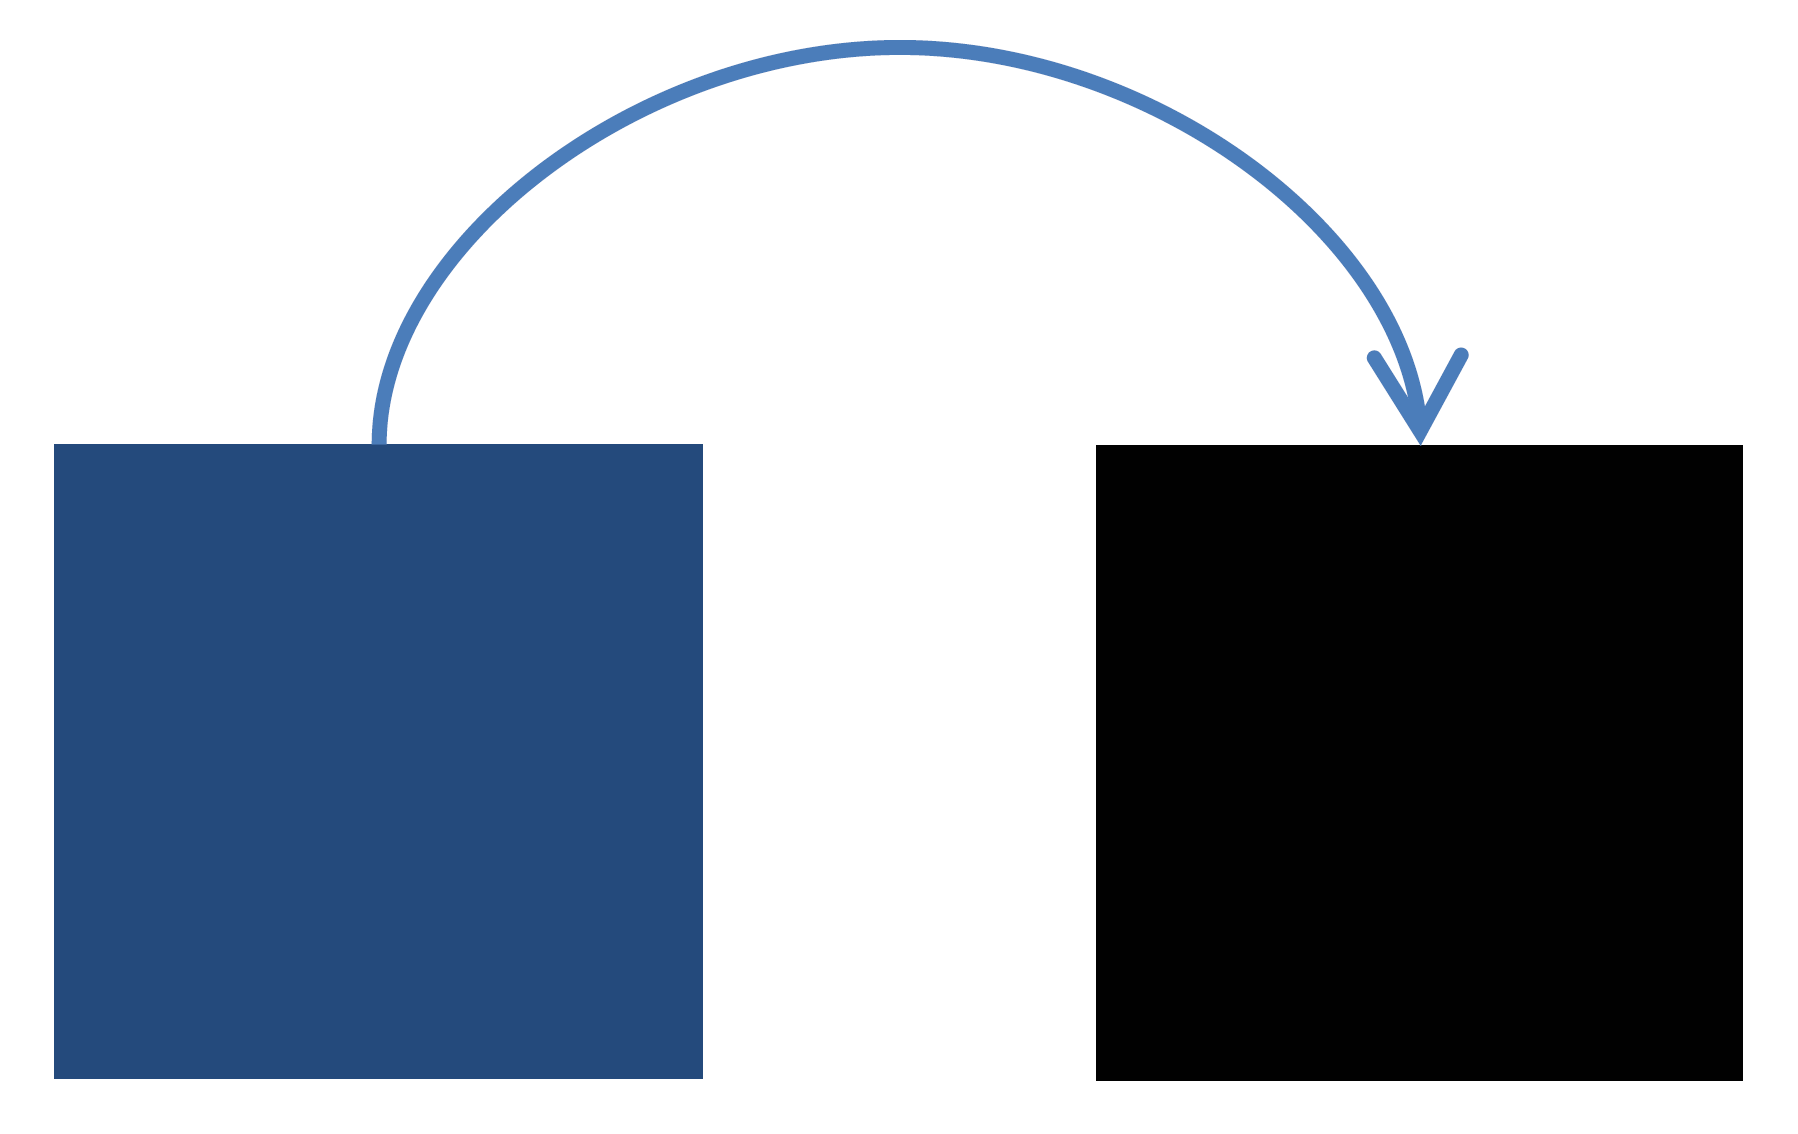
\includegraphics[width=0.2\linewidth, keepaspectratio=true]{images/intro/meta-learning.png}
	\end{center}
				
	\begin{itemize}
		\item Learning essentially never stops:
		\begin{itemize}
			\item Many models are periodically re-fit to track changes in the data
			\item Many models are re-fit to perform well on new tasks
		\end{itemize}
		\item The best hyperparameter configuration tends to remain quite stable across tasks
	\end{itemize}
	\bigskip
	\bigskip
	\bigskip
\pause
	\begin{center}
	For a good introduction to meta-learning in general, see \lit{\href{https://www.automl.org/wp-content/uploads/2019/05/AutoML_Book.pdf\#page=46&zoom=auto,-103,613}{AutoML Book: Chapter 2}}
	\end{center}			
\end{frame}

\begin{frame}[c]{Problem Statement}
%	\myblock{Definition: meta-learning for HPO}{
		Given:
	    \begin{itemize}
	        \item a set of prior tasks: 
	        %(e.g., datasets): 
	        $t_{j} \in \mathcal{T}_{\text{meta}} \subset \mathcal{T}$,
	        \item a set of new tasks: 
	        %(e.g., datasets): 
	        $t_{\text{new}} \in \mathcal{T}$,
\pause
	        \item a set of learning algorithms, fully defined by $\theta_{i} \in \Theta$
\pause
	        \item a set of prior evaluations $\dataset_{\text{meta}}$ on $t_j \in \mathcal{T}_{\text{meta}}$%, where $\dataset_{i, j} = \cost(\theta_{i}, t_{j})$
	        \item a set of evaluations $\dataset_{\text{new}}$ on new task $t_{\text{new}}$
		\end{itemize}
		\bigskip
\pause
		\alert{Goal of meta-learning:}
		\begin{itemize}
			\item use meta-data $\mathcal{D}_{\text{meta}}$ to choose $\theta_{i} \in \Theta$ for $t_{\text{new}}$ better than only based on $\dataset_{\text{new}}$. 
		\end{itemize}
%	}	
\bigskip
\hspace{9cm}\lit{\href{https://www.automl.org/wp-content/uploads/2019/05/AutoML_Book.pdf\#page=46&zoom=auto,-103,613}{adapted from AutoML Book: Chapter 2}}
\end{frame}


% %----------------------------------------------------------------------
% %----------------------------------------------------------------------
% \begin{frame}[c]{Meta-Learning}
% \framesubtitle{Introduction}

% \begin{columns}
% 	\column{0.18\textwidth}
% 	Ren\'e Magritte
% 	\centering
% 	
\includegraphics[width=.9\textwidth]{../w07_hpo_speedup/images/meta_learning/magritte_1.jpg}
% 	
\includegraphics[width=.9\textwidth]{../w07_hpo_speedup/images/meta_learning/magritte_2.jpg}
% 	\column{0.258\textwidth}
% 	Francis Picabia
% 	\centering
% 	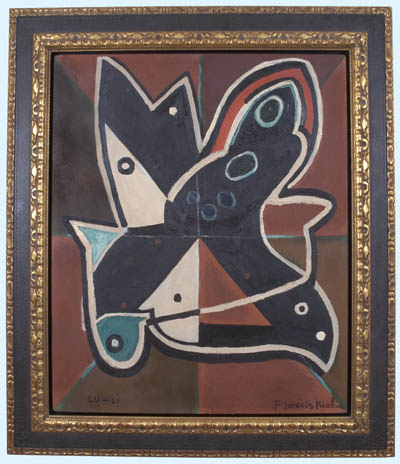
\includegraphics[width=.7\textwidth]{../w07_hpo_speedup/images/meta_learning/picabia_3.jpg}
% 	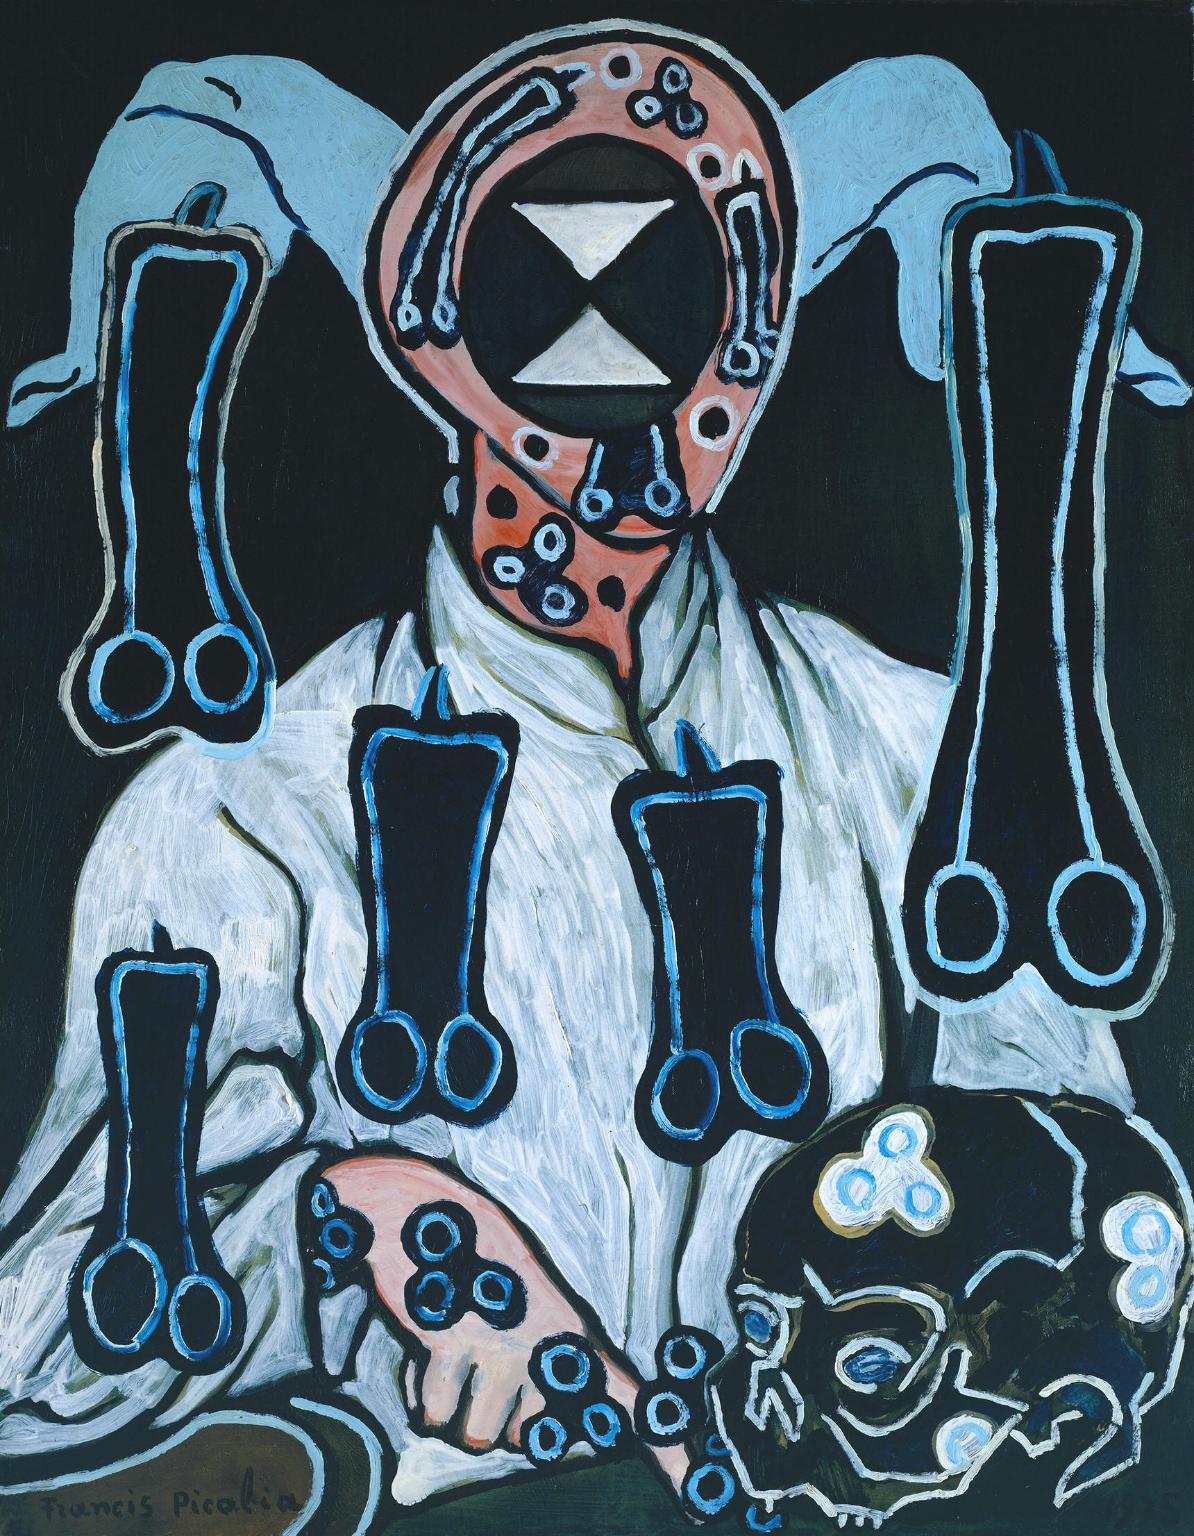
\includegraphics[width=.6\textwidth]{../w07_hpo_speedup/images/meta_learning/picabia_1.jpg}
% 	\column{0.3\textwidth}
% 	\centering
% 	Who painted that?
% 	
\includegraphics[width=.7\textwidth]{../w07_hpo_speedup/images/meta_learning/magritte_3.jpg}
	
% 	\fhpause
% 	Most likely most of you can identify the painter correctly, 
% 	although I presented only two pictures of each.
% \end{columns}

% \end{frame}
% % %----------------------------------------------------------------------
% % %----------------------------------------------------------------------

%----------------------------------------------------------------------
%----------------------------------------------------------------------
%\begin{frame}[c]{Learning from model evaluations}
%
%\begin{itemize}
%    \item Similarly, while building ML models for a specific task, we exploit our experience with related tasks
%    \item The challenge of meta-learning is to provide a systematic and data-driven approach to learn from experience 
%\end{itemize}
%
%\hspace{11cm}\lit{\href{https://www.springer.com/gp/book/9783030053178}{AutoML Book: Chapter 2}}
%
%\end{frame}
% %----------------------------------------------------------------------
% %----------------------------------------------------------------------

%----------------------------------------------------------------------
%----------------------------------------------------------------------
\begin{frame}[c]{The Role of Meta-Features}

\begin{itemize}
    \item We can often extract additional characteristics for each task, called \alert{meta-features}
    \item Each task $t_j$ can be described by a vector of $K$ meta-features:
        \begin{equation*}
            m(t_j) = (m_{j, 1}, \dots, m_{j, K})
        \end{equation*}
\medskip
\pause
    \item This vector can be used to define a \alert{similarity measure} between two tasks
    \begin{itemize}
    	\item e.g., calculating the Euclidean distance between $m(t_i)$ and $m(t_j)$
\smallskip
	    \item Based on similarity, we can transfer information from the most similar tasks to new task $t_{\text{new}}$
	\end{itemize}
\end{itemize}

\end{frame}
% %----------------------------------------------------------------------
% %----------------------------------------------------------------------

% \begin{frame}[c]{Meta-Learning}
% \framesubtitle{Supervised Learning revisited}

% Dataset:
% \begin{equation*}
% \dataset = \{(x_1, y_1), \ldots, (x_k, y_k) \}
% \end{equation*}

% \bigskip
% \fhpause

% Learning a model $\phi$ (e.g., weights of a neural network):
% \begin{eqnarray*}
% \argmax_{\phi} \log p(\phi|\dataset)\\
% \fhpause
% = \argmax_{\phi} \log p(\dataset | \phi) + \log p(\phi) \\
% \fhpause
% = \argmax_{\phi} \sum_i \log p(y_i | x_i, \phi) + \log p(\phi)
% \end{eqnarray*}

% \fhpause

% Challenge:
% \begin{itemize}
% 	\item Learning starts from scratch
% 	\item We might only have very few examples in $\dataset$ 
% \end{itemize}

% \end{frame}
% %----------------------------------------------------------------------
% %----------------------------------------------------------------------
% \begin{frame}[c]{Meta-Learning}
% \framesubtitle{Problem formulation}

% Dataset:
% \begin{equation*}
% \dataset = \{(x_1, y_1), \ldots, (x_k, y_k) \}
% \end{equation*}
% Set of datasets (meta-datasets):
% \begin{equation*}
% \mdata = \{\mathcal{D}_1, \ldots, \mathcal{D}_n, \}
% \end{equation*}

% \fhpause
% Can we include these meta-datasets to improve learning on $\dataset$?
% \begin{equation*}
% \argmax_{\phi} \log p(\phi|\dataset, \mdata)
% \end{equation*}

% \fhpause
% \medskip

% \alert{Idea:} Instead of keeping $\mdata$ forever, we want to distill the knowledge into \alert{meta-parameters $\theta$}: $p(\theta|\mdata)$
 
% \end{frame}
% %----------------------------------------------------------------------
% %----------------------------------------------------------------------
% \begin{frame}[c]{Meta-Learning}
% \framesubtitle{Problem formulation}

% In meta-learning, we want to learn:
% \begin{eqnarray*}
% \argmax_{\phi} \log p(\phi|\dataset, \mdata) \\
% \fhpause
% = \argmax_{\phi} \log \int_{\Theta} p(\phi \mid \dataset, \theta) p(\theta \mid \mdata) d\theta\\
% \fhpause
% \approx \argmax_{\phi} \log p(\phi | \dataset, \theta^*) + \log p(\theta^* | \mdata)\\
% \fhpause
% = \argmax_{\phi} \log p(\phi | \dataset, \theta^*)
% \end{eqnarray*}

% \fhpause

% \begin{center}
% \begin{minipage}{0.5\textwidth}
% \begin{block}{Meta-learning problem}
% \begin{equation*}
% \theta^* \in \argmax_{\theta} \log p(\theta | \mdata)
% \end{equation*}
% \end{block}
% \end{minipage}
% \end{center}

% \end{frame}
% %-----------------------------------------------------------------------
% %-----------------------------------------------------------------------
% \begin{frame}[c]{Meta-Learning}
% \framesubtitle{AutoML $\subset$ Meta-Learning}

% \begin{itemize}
% 	\item AutoML can be seen as a special case of meta-learning \fhpause
% 	\medskip
% 	\item $\theta$ could be:
% 	\begin{itemize}
% 		\item a hyperparameter configuration ($\lambda$) 
% 		\item a neural network architecture
% 	\end{itemize}
% 	\fhpause
% 	\medskip
% 	\item What would be $\mdata$ here? 
% 	\fhpause
% 	\begin{itemize}
% 		\item A dataset on which we optimized $\lambda$ (e.g. CIFAR-10)\\ such that we can use it on another dataset (e.g. imagenet)
% 	\end{itemize}
% \end{itemize}	

% \end{frame}
% %-----------------------------------------------------------------------
% %-----------------------------------------------------------------------
% \begin{frame}[c]{Meta-Learning}
% \framesubtitle{Meta-Learning $\subset$ AutoML}

% \begin{itemize}
% 	\item Meta-learning can be powerful to complement AutoML
% 	\fhpause
% 	\medskip
% 	\item We can learn a lot of things from $\mdata$ to improve the performance on new datasets, e.g.:
% 	\begin{itemize}
% 		\item pre-initialization of networks weights
% 		\item learning a meta-DNN to predict how to train another target-DNN	\end{itemize}
% \end{itemize}	

% \end{frame}
%-----------------------------------------------------------------------
%-----------------------------------------------------------------------
\begin{frame}[c]{Overview of Meta-Features in Machine Learning}

\begin{itemize}
	\item \alert{Simple} - easily extracted from the data, describe the basic dataset structure
	\begin{itemize}
		\item e.g., number of features, data points or classes
		\pause
	\end{itemize}
	
	\item \alert{Statistical} - characterize the data via descriptive statistics:
	\begin{itemize}
		\item e.g., average or standard deviation of features, or their correlation with the labels
		\pause
	\end{itemize} 	
	\item \alert{Information-theoretic} - measure the class entropy in the data
	\begin{itemize}
		\item capture the amount of information in the data %and their complexity
		\pause 
    \end{itemize}
    \item \alert{Model-based} - extracted from a model induced using the training data
    \begin{itemize}
    	\item these are often based on properties of decision tree models
    	\item e.g., number of leaves, number of nodes, shape of the tree 
    	\pause
	\end{itemize}	
	\item \alert{Landmarking} - computed by running several fast ML algorithms on the dataset
	\begin{itemize}
		\item e.g., is fast algorithm A better than fast algorithm B on this dataset?
		\item this can capture different properties of the dataset, e.g., linear separability
		\pause
	\end{itemize}
	\item \alert{Others} - not included in the previous groups
	\begin{itemize}
		\item e.g., time related measures, clustering and distance-based measures
	\end{itemize}
	
\end{itemize}

\end{frame}
%-----------------------------------------------------------------------
%-----------------------------------------------------------------------
\begin{frame}[c]{Meta-Learning for HPO Approach 1: Warmstarting}
	
\begin{itemize}
	\item Experts often start HPO from a strong default (rather than random configurations)
	\pause
	\medskip
	\item Can we learn from meta-data $\mdata$ how to \alert{initialize} HPO?
	\pause
	\medskip
	\item Note: just a single default configuration often does not perform great on a new dataset
	\begin{itemize}
		\item Otherwise there would be no point in HPO
	\end{itemize}
	%, based on meta-features?
%	(i.e., running an initial design)
%	\begin{itemize}
%		\item the same ideas also apply to NAS
%		\item for simplicity we focus on HPO 
%	\end{itemize}
\end{itemize}

\end{frame}
%-----------------------------------------------------------------------
%----------------------------------------------------------------------
%----------------------------------------------------------------------
\begin{frame}[c]{Meta-Learning for HPO Approach 2: Model-Warmstarting}

\begin{itemize}
	\item Many HPO methods use a predictive model (e.g., Bayesian optimization)
	\medskip
	\item By running HPO on different datasets,
	we learn something about the search landscape
	\begin{itemize}
		\item E.g., what are bad regions of the configuration space in general
	\end{itemize}
	\bigskip
	\pause
	\item Given: $n$ predictive models $\surro_{\dataset_i}: \pcs \to \mathbb{R}$ from HPO on $\mathcal{T}_{\text{meta}}$	
	\item \alert{How can we use these $\surro_{\dataset_i}$ to speed up HPO?}
\end{itemize}


\end{frame}
%-----------------------------------------------------------------------

%-----------------------------------------------------------------------
%-----------------------------------------------------------------------
\myframetop{Meta-Learning for HPO Approach 3: Task-independent Recommendations}{

\begin{columns}[T] % align columns
\begin{column}{.48\textwidth}

\vspace*{-0.3cm}
    \onslide<1->{
    \begin{itemize}
        \item \emph{Idea:} learn a \alert{sorted list of defaults}
        \item \emph{Method:} mostly \alert{greedy} on $\mathcal{T}_{\text{meta}}$
        \item \emph{Results:} surprisingly strong,\\ better than Bayesian Optimization
    \end{itemize}}

    \onslide<2->{
    \begin{block}{Advantages}
    \begin{itemize}
    	\item Easy to share and use
    	\item Strong anytime performance
    	\item Embarrassingly parallel
    \end{itemize}
    \end{block}}
    
    \onslide<2->{
    \begin{block}{Disadvantages}
    \begin{itemize}
    	\item Not adaptive
    \end{itemize}
    \end{block}}

\end{column}%

\hfill%

\begin{column}{.48\textwidth}

    \centering
    \onslide<1->{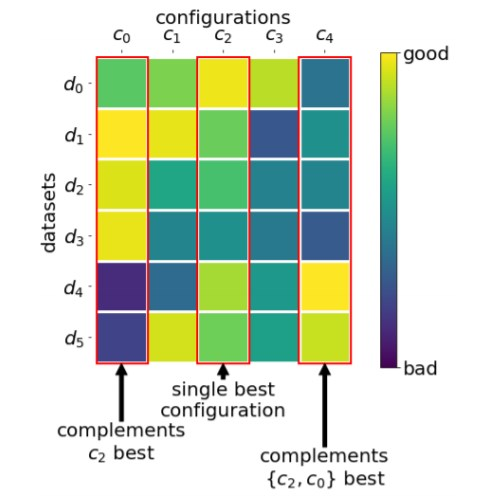
\includegraphics[width=.8\textwidth]{../w07_hpo_speedup/images/meta_learning/task_independent.jpg}}
%    \only<2->{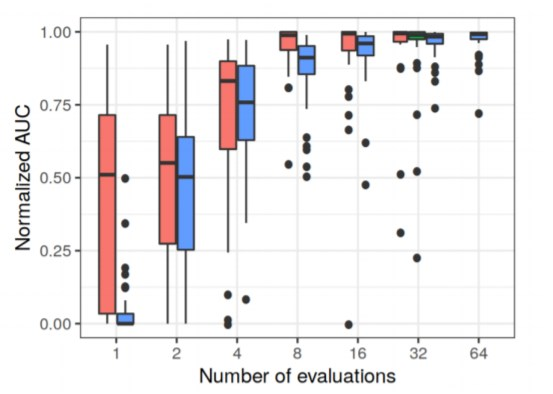
\includegraphics[width=.9\textwidth]{../w07_hpo_speedup/images/meta_learning/task_independent_results.jpg}}


\end{column}
\end{columns}  



\vspace{0.5cm}
\hspace{6cm}
\lit{\href{https://www.ismll.uni-hildesheim.de/pub/pdfs/scalable-gp-based-transfer-surrogates.pdf}{Wistuba et al. 2017}; \href{https://arxiv.org/pdf/1802.02219.pdf}{Feurer et al. 2018};  \href{https://arxiv.org/pdf/1811.09409.pdf}{Pfisterer et al. 2018}}

}
%-----------------------------------------------------------------------
%-----------------------------------------------------------------------

%-----------------------------------------------------------------------
%-----------------------------------------------------------------------
\begin{frame}[c]{Meta-Learning for HPO Approach 4:\\ Joint model for Bayesian optimization}

\begin{columns}[T] % align columns
\begin{column}{.38\textwidth}

\begin{itemize}
    \item<1-> \alert{Jointly train} a ``deep'' neural network \alert{on all tasks} 
    \myit{
    	\item<2-> Have a separate output layer (head) for each task 
    	\item<2-> Each head is a Bayesian linear regression (recall DNGO)
    }
    \item<3-> This uses meta-learning for feature extraction on the hyperparameter configurations 
\end{itemize}
\end{column}%

\hfill%

\begin{column}{.58\textwidth}
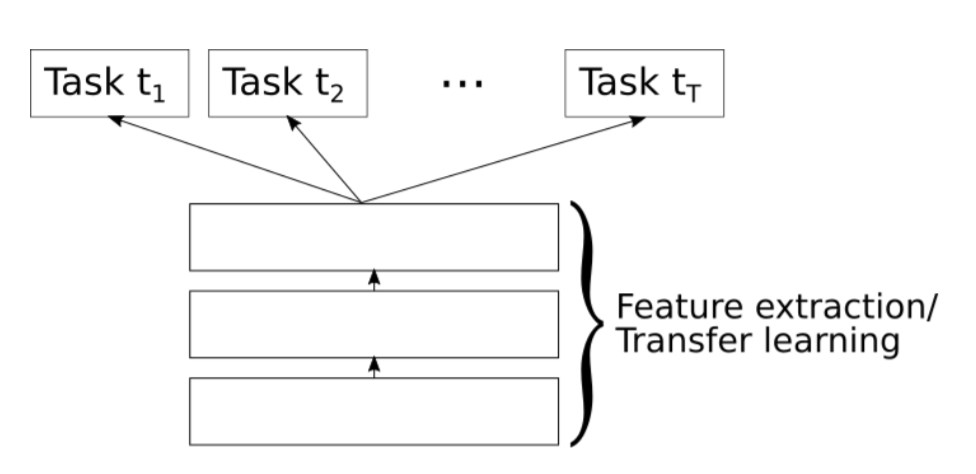
\includegraphics[width=0.9\textwidth]{../w07_hpo_speedup/images/meta_learning/perrone_int.jpg}
\end{column}%
\end{columns}

\hspace{12cm}\lit{\href{http://papers.nips.cc/paper/7917-scalable-hyperparameter-transfer-learning.pdf}{Perrone et al. 2018}}

\end{frame}
%-----------------------------------------------------------------------
%-----------------------------------------------------------------------
%\begin{frame}[c]{Joint model for Bayesian optimization}
%
%\centering
%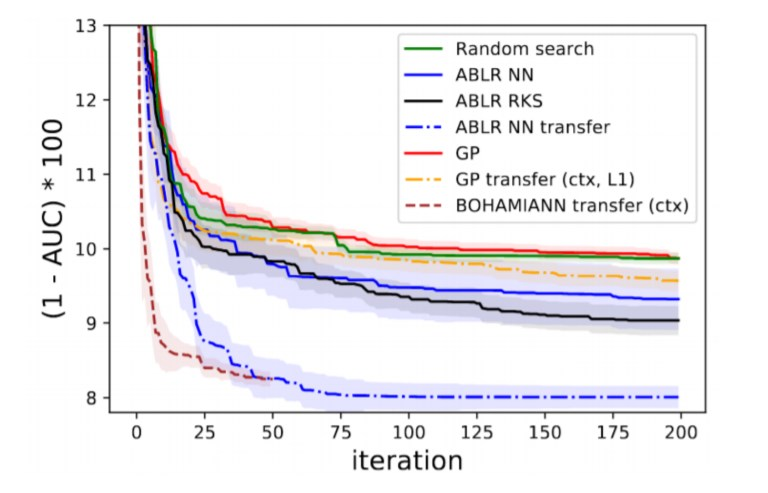
\includegraphics[width=0.7\textwidth]{../w07_hpo_speedup/images/meta_learning/perrone_res.jpg}
%
%\end{frame}
%-----------------------------------------------------------------------
%-----------------------------------------------------------------------

%----------------------------------------------------------------------
%----------------------------------------------------------------------
\begin{frame}[c]{Meta-Learning for HPO Approach 5:\\ Learning a Black-box Optimization Algorithm from Data}

\begin{itemize}
    \item \alert{Learning} a blackbox optimization algorithm
    \begin{itemize}
        \item Use $\dataset_{\text{meta}}$ to learn a mapping from $\dataset_{\text{new}}$ to the next configuration $\conf$ to evaluate
 %       \item This 
%        \item 
%        \cost_{i, \text{new}}$ on a new task $t_{\text{new}}$
 %       
 %       \iter[\bocount]{h}$ to next query $\iter[\bocount]{x}$
        \item This mapping can be a (recurrent) neural net $\text{NN}_{\phi}: \dataset_{\text{new}} \mapsto \conf$ parameterized by weights $\phi$   
\pause        
\smallskip
        \item \alert{This mapping $\text{NN}_{\phi}$ constitutes a blackbox optimization algorithm}
%        \myit{
%            \item Should be learned on a \alert{meta-train} set of blackbox functions \& generalize to new functions
%            \item Like a manually-designed algorithm ...
%        }

%\fhpause
%        \item Since $\iter[\bocount]{h}$ captures a \alert{sequence}, a recurrent NN $RNN_{\phi}:\iter[\bocount]{h} \mapsto \iter[\bocount]{x}$ makes sense

\pause
\bigskip
    
    \end{itemize}
    
    \item Existing approaches for learning a blackbox optimizer

    \begin{itemize}
        \item \alert{Gradient descent} on $\phi$  \lit{\href{https://arxiv.org/pdf/1611.03824.pdf}{Chen et al. 2016}}
        \begin{itemize}
            \item Simplest technique, but requires backpropagation through the optimization trace
            \item This also requires the blackbox functions $f$ used for training to be differentiable
       \end{itemize}
\pause
        \item \alert{Reinforcement learning} \lit{\href{https://arxiv.org/pdf/1606.01885.pdf}{Li and Malik. 2016}}
        \begin{itemize}

            \item Can be harder to get to work, but does not require differentiable $f$
        \end{itemize}
    
%        \item Gradient-free approaches should also work

    \end{itemize}
\end{itemize}

\end{frame}
%----------------------------------------------------------------------
%----------------------------------------------------------------------
%-----------------------------------------------------------------------
%-----------------------------------------------------------------------
\begin{frame}[c]{Meta-Learning for HPO Approach 6: Learning Algorithm Parts}

\begin{itemize}
	\item Learning a complete optimization algorithm  \alert{requires a lot of data}
	\item It would be more \alert{sample-efficient} to \alert{only replace hand-designed parts} of an algorithm

\bigskip
\pause
	\item In Bayesian optimization, a critical hand-designed heuristic is the acquisition function
	\begin{itemize}
		\item Trade-off between exploitation and exploration, e.g., via PI, EI, UCB, ES, KG, \dots 
		\item Depending on the problem at hand, you might need a different acquisition function
		%all of them are \alert{myopic} (no long-term look-ahead)
	\end{itemize}
\pause
\smallskip

    \item \alert{Idea:} Learn a \alert{neural acquisition function} from data, but still make use of the sample efficiency of Gaussian processes \lit{\href{https://openreview.net/pdf?id=ryeYpJSKwr}{Volpp et al. 2019}}

\pause
\medskip
    \item Two options:
    \begin{itemize}
        \item Only depend on predicted mean and variance: $\acq_\phi(\conf) = \acq_\phi(\mu_t(\conf), \sigma_t(\conf))$ 
        \begin{itemize}
            \item This allows to learn a general acquisition function
        \end{itemize}
\pause
        \item Also depend on the $\conf$ value: $\acq_\phi(\conf) = \acq_\phi(\mu_t(\conf), \sigma_t(\conf), \alert{\conf})$  
        \begin{itemize}
            \item This allows to fine-tune to the characteristics of $\mathcal{D}_{\text{meta}}$ (e.g., avoid poor parts of the space) 
        \end{itemize}
    \end{itemize}

\end{itemize}


\end{frame}
%-----------------------------------------------------------------------

%-----------------------------------------------------------------------
\begin{frame}[c]{Questions to Answer for Yourself / Discuss with Friends}

\begin{itemize}
    \item \alert{Repetition.} What are the different kinds of meta-features which can be used to describe machine learning datasets?
    
    \medskip

    \item \alert{Repetition.} List all the different ways of using the meta data for HPO you recall
    \medskip

    \item \alert{Discussion.}
%        \item How would you pick meta-features to be used in meta-learning hyperparameter optimization?
        In the various meta-learning approaches, what will happen if all prior tasks are dissimilar to the target task?


\end{itemize}

\end{frame}
\end{document}